% This example is meant to be compiled with lualatex or xelatex
% The theme itself also supports pdflatex
\PassOptionsToPackage{unicode}{hyperref}
\documentclass[aspectratio=1610, 12pt, xcolor=dvipsnames]{beamer}

% Warning, if another latex run is needed
% \usepackage[aux]{rerunfilecheck}

% just list chapters and sections in the toc, not subsections or smaller
\setcounter{tocdepth}{1}

%------------------------------------------------------------------------------
%------------------------------ Fonts, Unicode, Language ----------------------
%------------------------------------------------------------------------------
\usepackage{fontspec}
\defaultfontfeatures{Ligatures=TeX}  % -- becomes en-dash etc.

% german language
\usepackage{polyglossia}
\setdefaultlanguage{german}

% for english abstract and english titles in the toc
\setotherlanguages{english}

% intelligent quotation marks, language and nesting sensitive
\usepackage[autostyle]{csquotes}

% microtypographical features, makes the text look nicer on the small scale
\usepackage{microtype}

% colors and stuff
\usepackage{xcolor}
\usepackage[most]{tcolorbox}
% Here was colback=SpringGreen before but it is not finding the xcolor package
\tcbset{on line,
        boxsep=4pt, left=0pt,right=0pt,top=0pt,bottom=0pt,
        colframe=white,colback=green,
        highlight math style={enhanced}
        }
\newtcolorbox{mybox}[3][]
{
  colframe = #2!25,
  colback = #2!20,
  coltitle = #2!20!black,
  title = {#3},
  #1
}
%\colorlet{Green!40}
%------------------------------------------------------------------------------
%------------------------ Math Packages and settings --------------------------
%------------------------------------------------------------------------------

\usepackage{amsmath}
\usepackage{amssymb}
\usepackage{mathtools}
\usepackage{bbold}

% Enable Unicode-Math and follow the ISO-Standards for typesetting math
\usepackage[
  math-style=ISO,
  bold-style=ISO,
  sans-style=italic,
  nabla=upright,
  partial=upright,
]{unicode-math}
\setmathfont{Latin Modern Math}

% nice, small fracs for the text with \sfrac{}{}
\usepackage{xfrac}


%------------------------------------------------------------------------------
%---------------------------- Numbers and Units -------------------------------
%------------------------------------------------------------------------------

\usepackage[
  locale=DE,
  separate-uncertainty=true,
  per-mode=symbol-or-fraction,
]{siunitx}
\sisetup{math-micro=\text{µ},text-micro=µ}
% \sisetup{tophrase={{ to }}}
%------------------------------------------------------------------------------
%-------------------------------- tables  -------------------------------------
%------------------------------------------------------------------------------

\usepackage{booktabs}       % \toprule, \midrule, \bottomrule, etc

%------------------------------------------------------------------------------
%-------------------------------- graphics -------------------------------------
%------------------------------------------------------------------------------

\usepackage{graphicx}
%\usepackage{rotating}
\usepackage{grffile}
\usepackage{tikz}
\usepackage{circuitikz}
\usepackage{tikz-feynman}
\usepackage{subcaption}

% allow figures to be placed in the running text by default:
\usepackage{scrhack}
\usepackage{float}
\floatplacement{figure}{htbp}
\floatplacement{table}{htbp}

% keep figures and tables in the section
\usepackage[section, below]{placeins}

% smileys
\usepackage{MnSymbol,wasysym}

%------------------------------------------------------------------------------
%---------------------- customize list environments ---------------------------
%------------------------------------------------------------------------------

\usepackage{enumitem}
\usepackage{listings}
\usepackage{hepunits}

\usepackage{pdfpages}
%------------------------------------------------------------------------------
%------------------------------ Bibliographie ---------------------------------
%------------------------------------------------------------------------------

\usepackage[
  backend=biber,   % use modern biber backend
  autolang=hyphen, % load hyphenation rules for if language of bibentry is not
                   % german, has to be loaded with \setotherlanguages
                   % in the references.bib use langid={en} for english sources
]{biblatex}
\addbibresource{references.bib}  % the bib file to use
\DefineBibliographyStrings{german}{andothers = {{et\,al\adddot}}}  % replace u.a. with et al.


% Load packages you need here
% \usepackage{polyglossia}
% \setmainlanguage{german}

\usepackage{csquotes}


% \usepackage{amsmath}
% \usepackage{amssymb}
% \usepackage{mathtools}

\usepackage{hyperref}
\usepackage{bookmark}

% load the theme after all packages

\usetheme[
  showtotalframes, % show total number of frames in the footline
]{tudo}

% Put settings here, like
\unimathsetup{
  math-style=ISO,
  bold-style=ISO,
  nabla=upright,
  partial=upright,
  mathrm=sym,
}

% \setbeamertemplate{itemize item}{\scriptsize$\blacktriangleright$}
% \setbeamertemplate{itemize subitem}{\scriptsize$\blacktriangleright$}

%Titel:
\title{Bachelorseminar: Detektorsysteme und Hardwareprojekte}
%Autor
\author[N.Breer]{\textbf{Nils Breer}}
%Lehrstuhl/Fakultät
\institute{TU Dortmund}
%Titelgrafik muss ich einfueren!!!
%\titlegraphic{\includegraphics[width=0.3\textwidth]{content/Bilder/interferenz.jpg}}
\date{18.04.2023}

\begin{document}
\maketitle

\begin{frame}\frametitle{Vertex Locator (VELO)}
  \begin{itemize}
    \item $\bullet$\,
    \item $\bullet$\,
    \item $\bullet$\,
  \end{itemize}
\end{frame}

\begin{frame}\frametitle{Scintillating Fibre Tracker (SciFi)}
  \begin{itemize}
    \item $\bullet$\,
    \item $\bullet$\,
    \item $\bullet$\,
  \end{itemize}
\end{frame}

\begin{frame}\frametitle{Upstream Tracker (UT)}
  \begin{itemize}
    \item $\bullet$\,
    \item $\bullet$\,
    \item $\bullet$\,
  \end{itemize}
\end{frame}

\begin{frame}\frametitle{Ring Immaging Cherenkov Detector}
  \begin{itemize}
    \item $\bullet$\,
    \item $\bullet$\,
    \item $\bullet$\,
  \end{itemize}
\end{frame}

\begin{frame}\frametitle{LumiTracker}
  \begin{itemize}
    \item $\bullet$\,
    \item $\bullet$\,
    \item $\bullet$\,
  \end{itemize}
\end{frame}

\begin{frame}\frametitle{TimePix4 Telescope}
  \begin{itemize}
    \item $\bullet$\,
    \item $\bullet$\,
    \item $\bullet$\,
  \end{itemize}
\end{frame}

\begin{frame}\frametitle{Beam Conditions Monitor (BCM)}
  \begin{itemize}
    \item $\bullet$\,
    \item $\bullet$\,
    \item $\bullet$\,
  \end{itemize}
\end{frame}

\begin{frame}\frametitle{BCM40 boards}
  \begin{itemize}
    \item $\bullet$\,
    \item $\bullet$\,
    \item $\bullet$\,
  \end{itemize}
\end{frame}

\begin{frame}\frametitle{MIBAD boards}
  \begin{itemize}
    \item $\bullet$\,
    \item $\bullet$\,
    \item $\bullet$\,
  \end{itemize}
\end{frame}

\begin{frame}\frametitle{Diamond RnD}
  \begin{itemize}
    \item $\bullet$\,
    \item $\bullet$\,
    \item $\bullet$\,
  \end{itemize}
\end{frame}

\begin{frame}\frametitle{FPGAs}
  \begin{itemize}
    \item $\bullet$\,
    \item $\bullet$\,
    \item $\bullet$\,
  \end{itemize}
\end{frame}

\begin{frame}\frametitle{}
  \begin{itemize}
    \item $\bullet$\,
    \item $\bullet$\,
    \item $\bullet$\,
  \end{itemize}
\end{frame}

\begin{frame}\frametitle{}
  \begin{itemize}
    \item $\bullet$\,
    \item $\bullet$\,
    \item $\bullet$\,
  \end{itemize}
\end{frame}

\begin{frame}\frametitle{}
  \begin{itemize}
    \item $\bullet$\,
    \item $\bullet$\,
    \item $\bullet$\,
  \end{itemize}
\end{frame}

\begin{frame}\frametitle{}
  \begin{itemize}
    \item $\bullet$\,
    \item $\bullet$\,
    \item $\bullet$\,
  \end{itemize}
\end{frame}

\begin{frame}\frametitle{}
  \begin{itemize}
    \item $\bullet$\,
    \item $\bullet$\,
    \item $\bullet$\,
  \end{itemize}
\end{frame}

\begin{frame}\frametitle{}
  \begin{itemize}
    \item $\bullet$\,
    \item $\bullet$\,
    \item $\bullet$\,
  \end{itemize}
\end{frame}

\begin{frame}\frametitle{}
  \begin{itemize}
    \item $\bullet$\,
    \item $\bullet$\,
    \item $\bullet$\,
  \end{itemize}
\end{frame}

\begin{frame}\frametitle{}
  \begin{itemize}
    \item $\bullet$\,
    \item $\bullet$\,
    \item $\bullet$\,
  \end{itemize}
\end{frame}

\begin{frame}\frametitle{}
  \begin{itemize}
    \item $\bullet$\,
    \item $\bullet$\,
    \item $\bullet$\,
  \end{itemize}
\end{frame}

\begin{frame}\frametitle{}
  \begin{itemize}
    \item $\bullet$\,
    \item $\bullet$\,
    \item $\bullet$\,
  \end{itemize}
\end{frame}

\begin{frame}\frametitle{}
  \begin{itemize}
    \item $\bullet$\,
    \item $\bullet$\,
    \item $\bullet$\,
  \end{itemize}
\end{frame}

\begin{frame}\frametitle{}
  \begin{itemize}
    \item $\bullet$\,
    \item $\bullet$\,
    \item $\bullet$\,
  \end{itemize}
\end{frame}

\begin{frame}\frametitle{}
  \begin{itemize}
    \item $\bullet$\,
    \item $\bullet$\,
    \item $\bullet$\,
  \end{itemize}
\end{frame}

\begin{frame}\frametitle{}
  \begin{itemize}
    \item $\bullet$\,
    \item $\bullet$\,
    \item $\bullet$\,
  \end{itemize}
\end{frame}

\begin{frame}\frametitle{}
  \begin{itemize}
    \item $\bullet$\,
    \item $\bullet$\,
    \item $\bullet$\,
  \end{itemize}
\end{frame}

\begin{frame}\frametitle{}
  \begin{itemize}
    \item $\bullet$\,
    \item $\bullet$\,
    \item $\bullet$\,
  \end{itemize}
\end{frame}

\begin{frame}\frametitle{}
  \begin{itemize}
    \item $\bullet$\,
    \item $\bullet$\,
    \item $\bullet$\,
  \end{itemize}
\end{frame}

\begin{frame}\frametitle{}
  \begin{itemize}
    \item $\bullet$\,
    \item $\bullet$\,
    \item $\bullet$\,
  \end{itemize}
\end{frame}

\begin{frame}\frametitle{}
  \begin{itemize}
    \item $\bullet$\,
    \item $\bullet$\,
    \item $\bullet$\,
  \end{itemize}
\end{frame}
% \begin{frame}\frametitle{Track hits comparison of V2 and simulation}
% \begin{mybox}{green}{}
%   \begin{itemize}
%     \item $\bullet$\, MC: hits on \textbf{reconstructed} tracks fill whole detector
%     \item $\bullet$\, data: filling tracks into A-side \to\, good!
%   \end{itemize}
% \end{mybox}
% \begin{mybox}{orange}{}
%   \begin{itemize}
%     \item \to\, scan C-side quarters for possible issues in distinct layers
%   \end{itemize}
% \end{mybox}
%   \begin{columns}
%     \begin{column}[c]{0.48\textwidth}
%       \begin{figure}
%         \centering
%         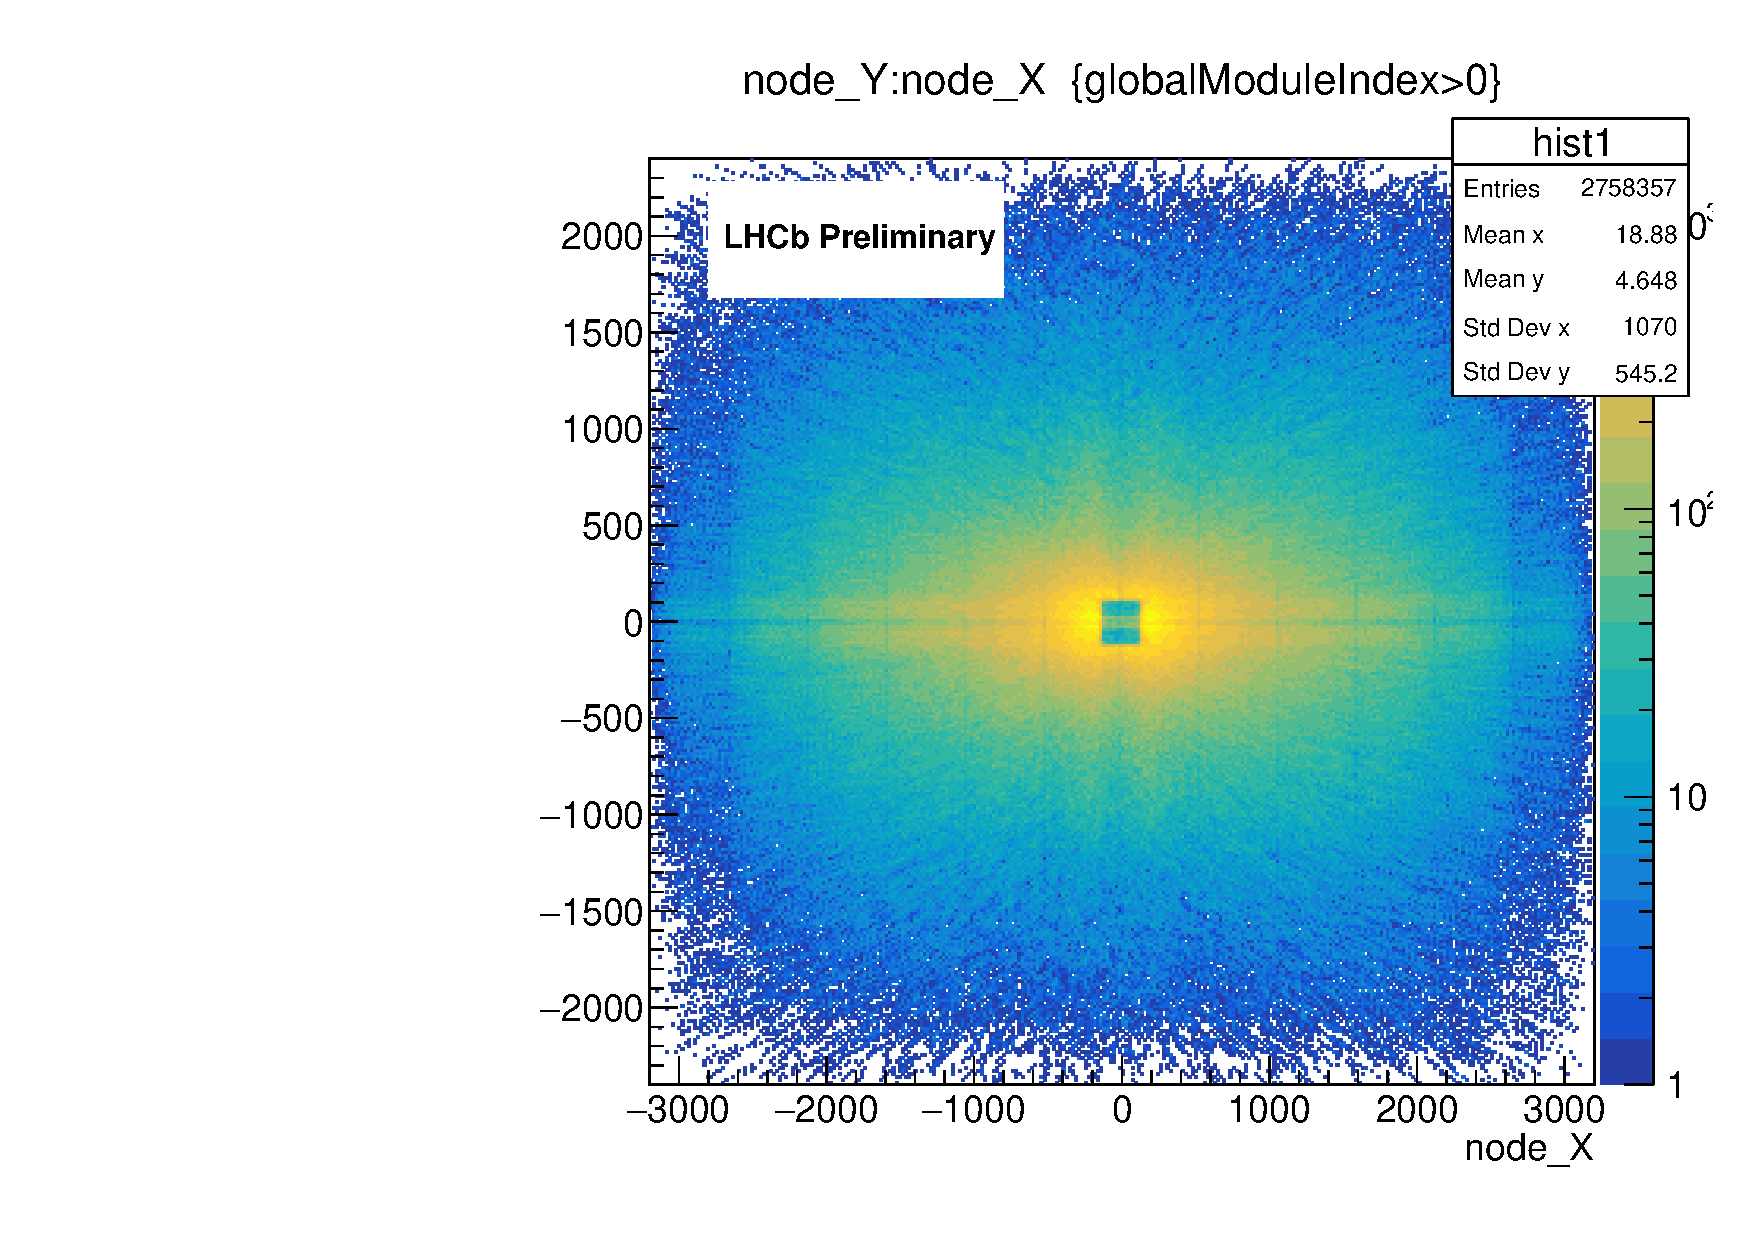
\includegraphics[width=0.6\textwidth]{logos/nodeXY_MC.pdf}%
%       \end{figure}
%     \end{column}
%     \begin{column}[c]{0.48\textwidth}
%       \begin{figure}
%         \centering
%         \includegraphics[width=0.6\textwidth]{tuples_out/combining_2D_nodeXY_v2.pdf}%
%       \end{figure}
%     \end{column}
%   \end{columns}
% \end{frame}

% \begin{frame}\frametitle{New Q0 positions in T2X2 layer}
%   \begin{itemize}
%     \item $\bullet$\, Changes based on V2 alignment positions
%     \item $\bullet$\, test incremental shifts of position/rotation until we found an improvement
%     \item $\bullet$\, rotations are with regard to the local frame of the module
%     \item $\bullet$\, positions: translations relative to the nominal position for each module
%     \item $\bullet$\, V2 alignment has only few tracks in Q0 because parts of the SciFi are too far out of alignment
%   \end{itemize}
%   \begin{figure}
%     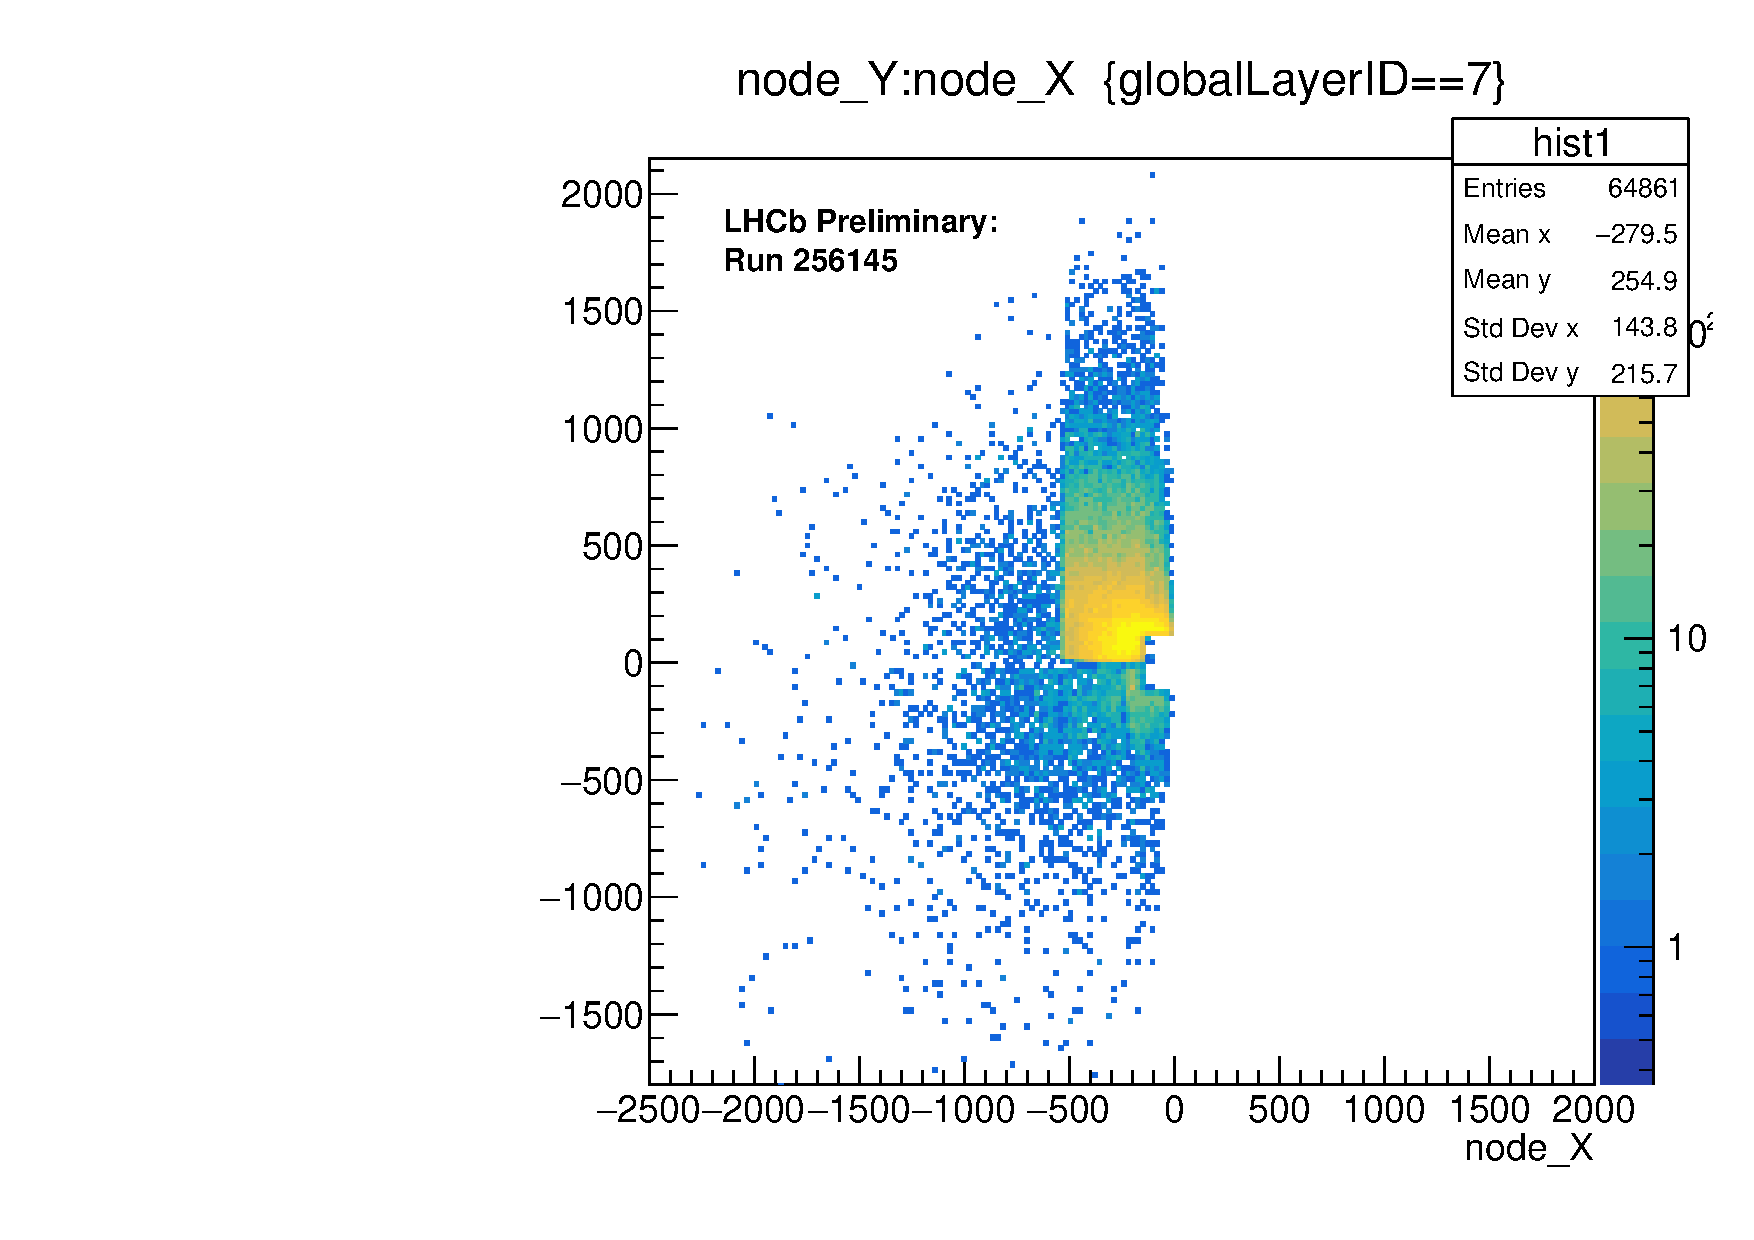
\includegraphics[width=0.26\textwidth]{logos/2D_nodeXY_v2_7_left.pdf}%
%     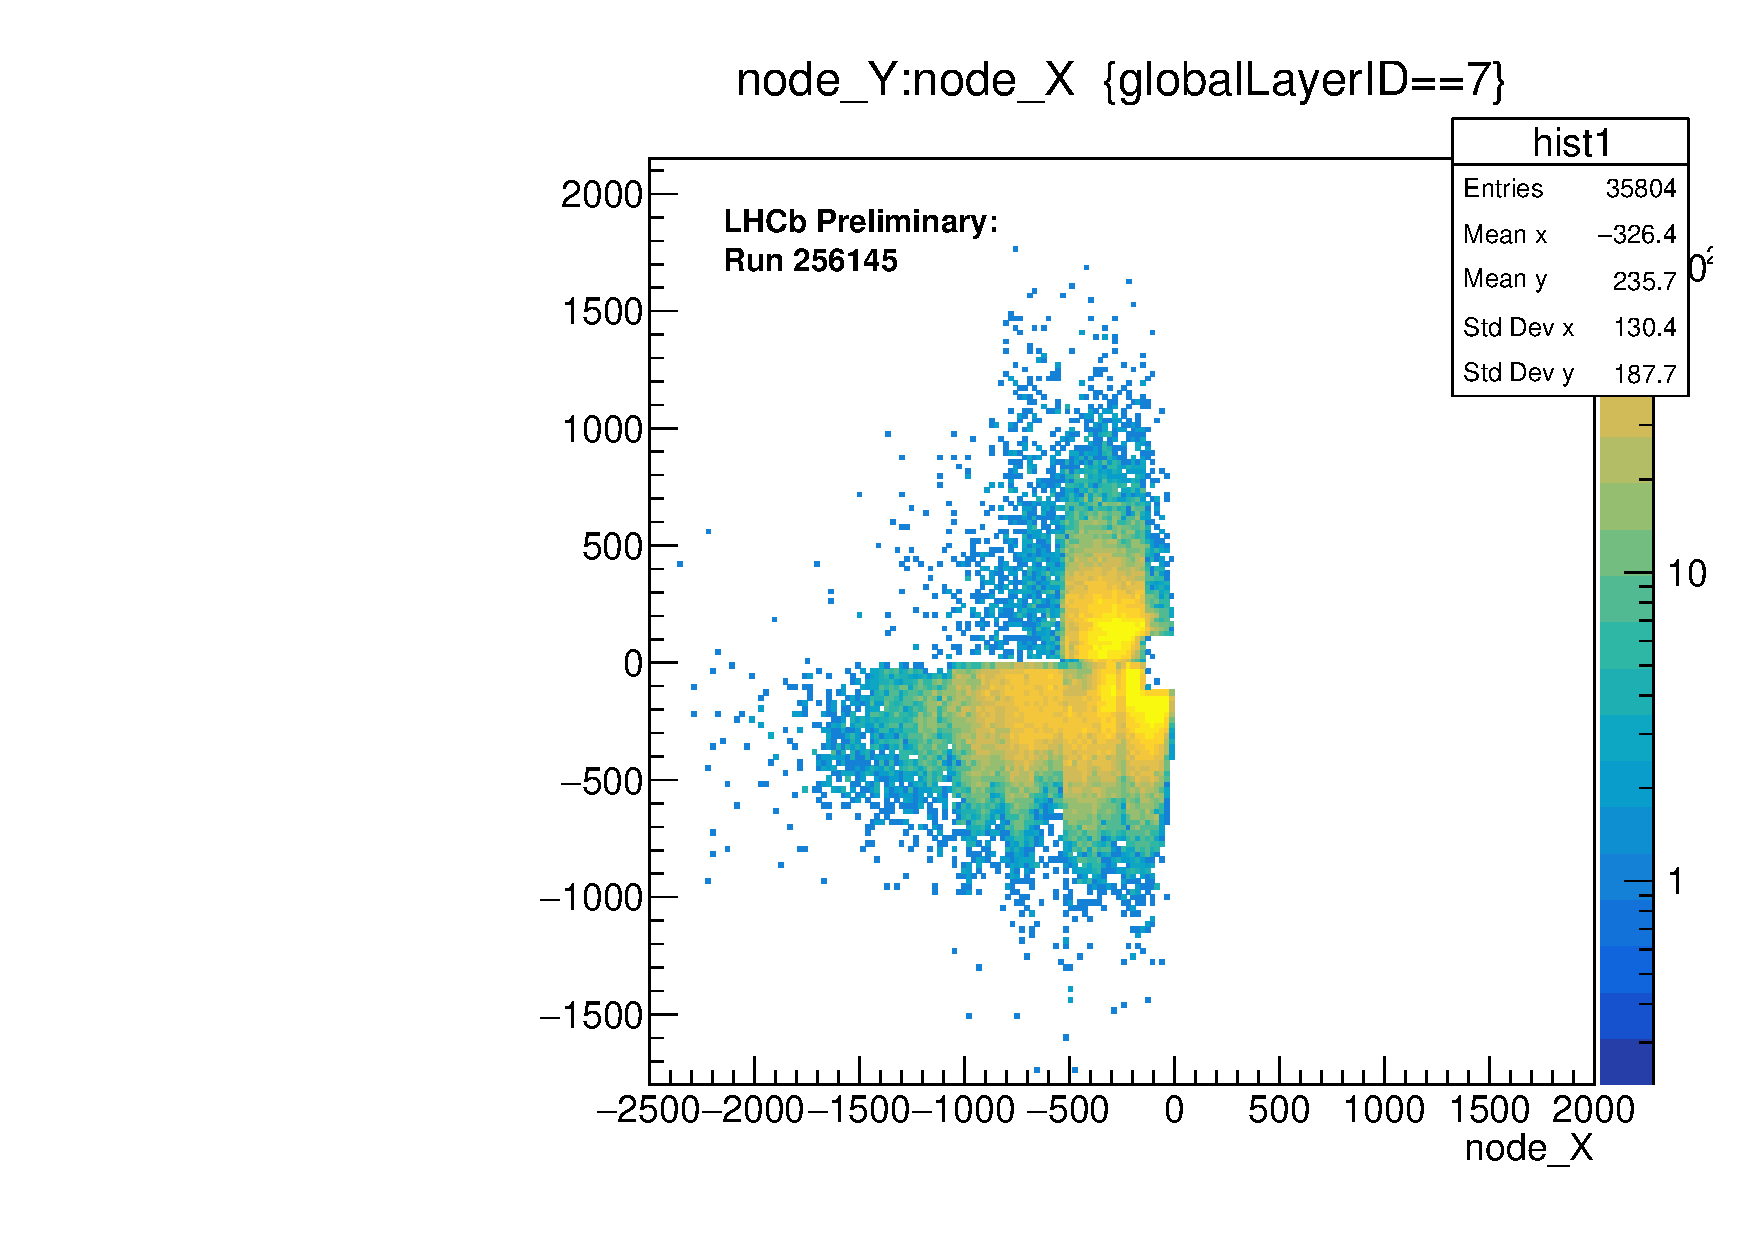
\includegraphics[width=0.26\textwidth]{logos/2D_nodeXY_quartermean_7_left.pdf}%
%     \includegraphics[width=0.26\textwidth]{problem_layer.png}%
%   \end{figure}
% \end{frame}

\end{document}
